\section{Проектирование и разработка архитектуры программного продукта}

После анализа требований к разрабатываемому продукту нужно составить все необходимые диаграммы, включая MindMap и UseCase.

\subsection{Построение диаграммы связей}

Для общей наглядности внутренностей проекта была составлена карта связей, она же MindMap, показанная на
рисунке \ref{des:mind_map}.

\begin{figure}[H]
    \center{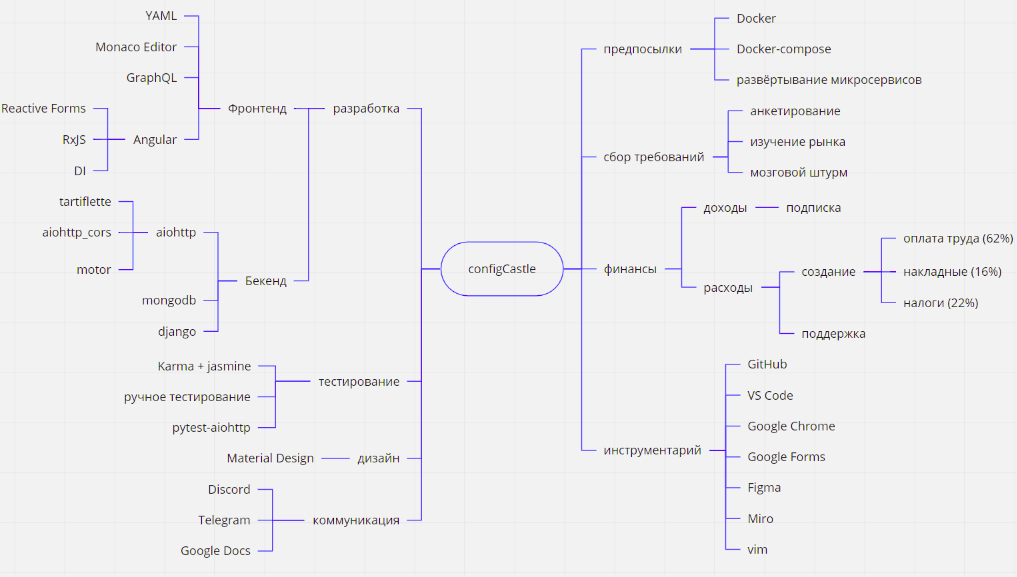
\includegraphics[scale=0.65]{mindmap.png}}
    \caption{Диаграмма связей}
    \label{des:mind_map}
\end{figure}

Здесь показана общая концепция продукта, что стало его предпосылкой, какие инструментальные средства использовались
и так далее.

В дальнейшем можно использовать эту карту, разместив её в wiki проекта для того, чтобы новые разработчики смогли ознакомиться с ней
и приступить к работе с минимальными затратами, понять какую проблему решает продукт, что используется для разработки, как происходит
коммуникация между разработчиками и с какими библиотеками необходимо быть знакомым.

\subsection{Разработка сценария использования}

После анализа ответов на вопрос можно прийти к определённым сценариям взаимодействия с пользователем. Исходя из принципа доступности и легко-понятного
пользовательского интерфейса, можно сконструировать определённые сценарии взаимодействия пользователей с программным продуктом. Результат подобной работы
изображен на так называемой диаграмме UseCase, привидённой на рисунке \ref{des:use_case}.

\begin{figure}[H]
    \center{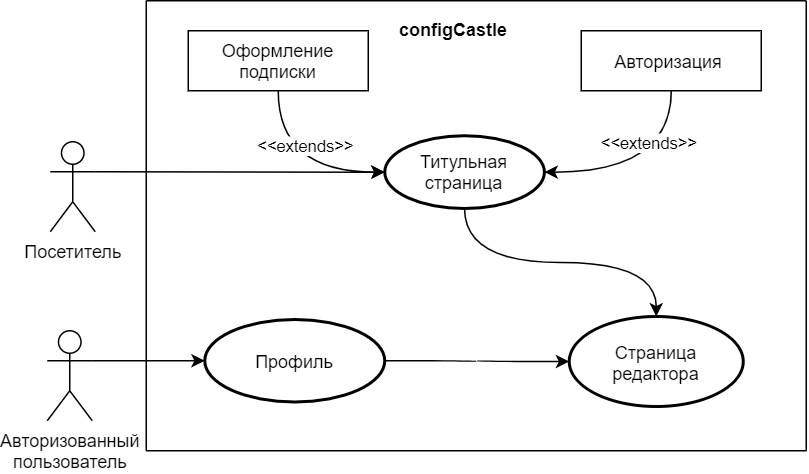
\includegraphics[scale=0.5]{usecase.png}}
    \caption{Диаграмма UseCase}
    \label{des:use_case}
\end{figure}

\subsection{Прототипирование и дизайн программного продукта}

На рисунках \ref{des:proto_1}, \ref{des:proto_2}, \ref{des:proto_3}, \ref{des:proto_4}, \ref{des:proto_5} и
\ref{des:proto_6} показаны прототипы, которые были созданы специально для проекта. Отображены и обозначены основные блоки дизайна, а также различия между
одними и теми же страницами, но с отличаюмещеся ролями пользователей. Так, например, пользователь с подпиской, т.е. клиент имеет функцию сохранить конфигурационный файл
в базе данных и использовать его в дальнейшем тогда как пользователь с ролью посетитель может только создать один файл в реальном времени, не имея возможности обозначенной ранее.

\begin{figure}[H]
    \center{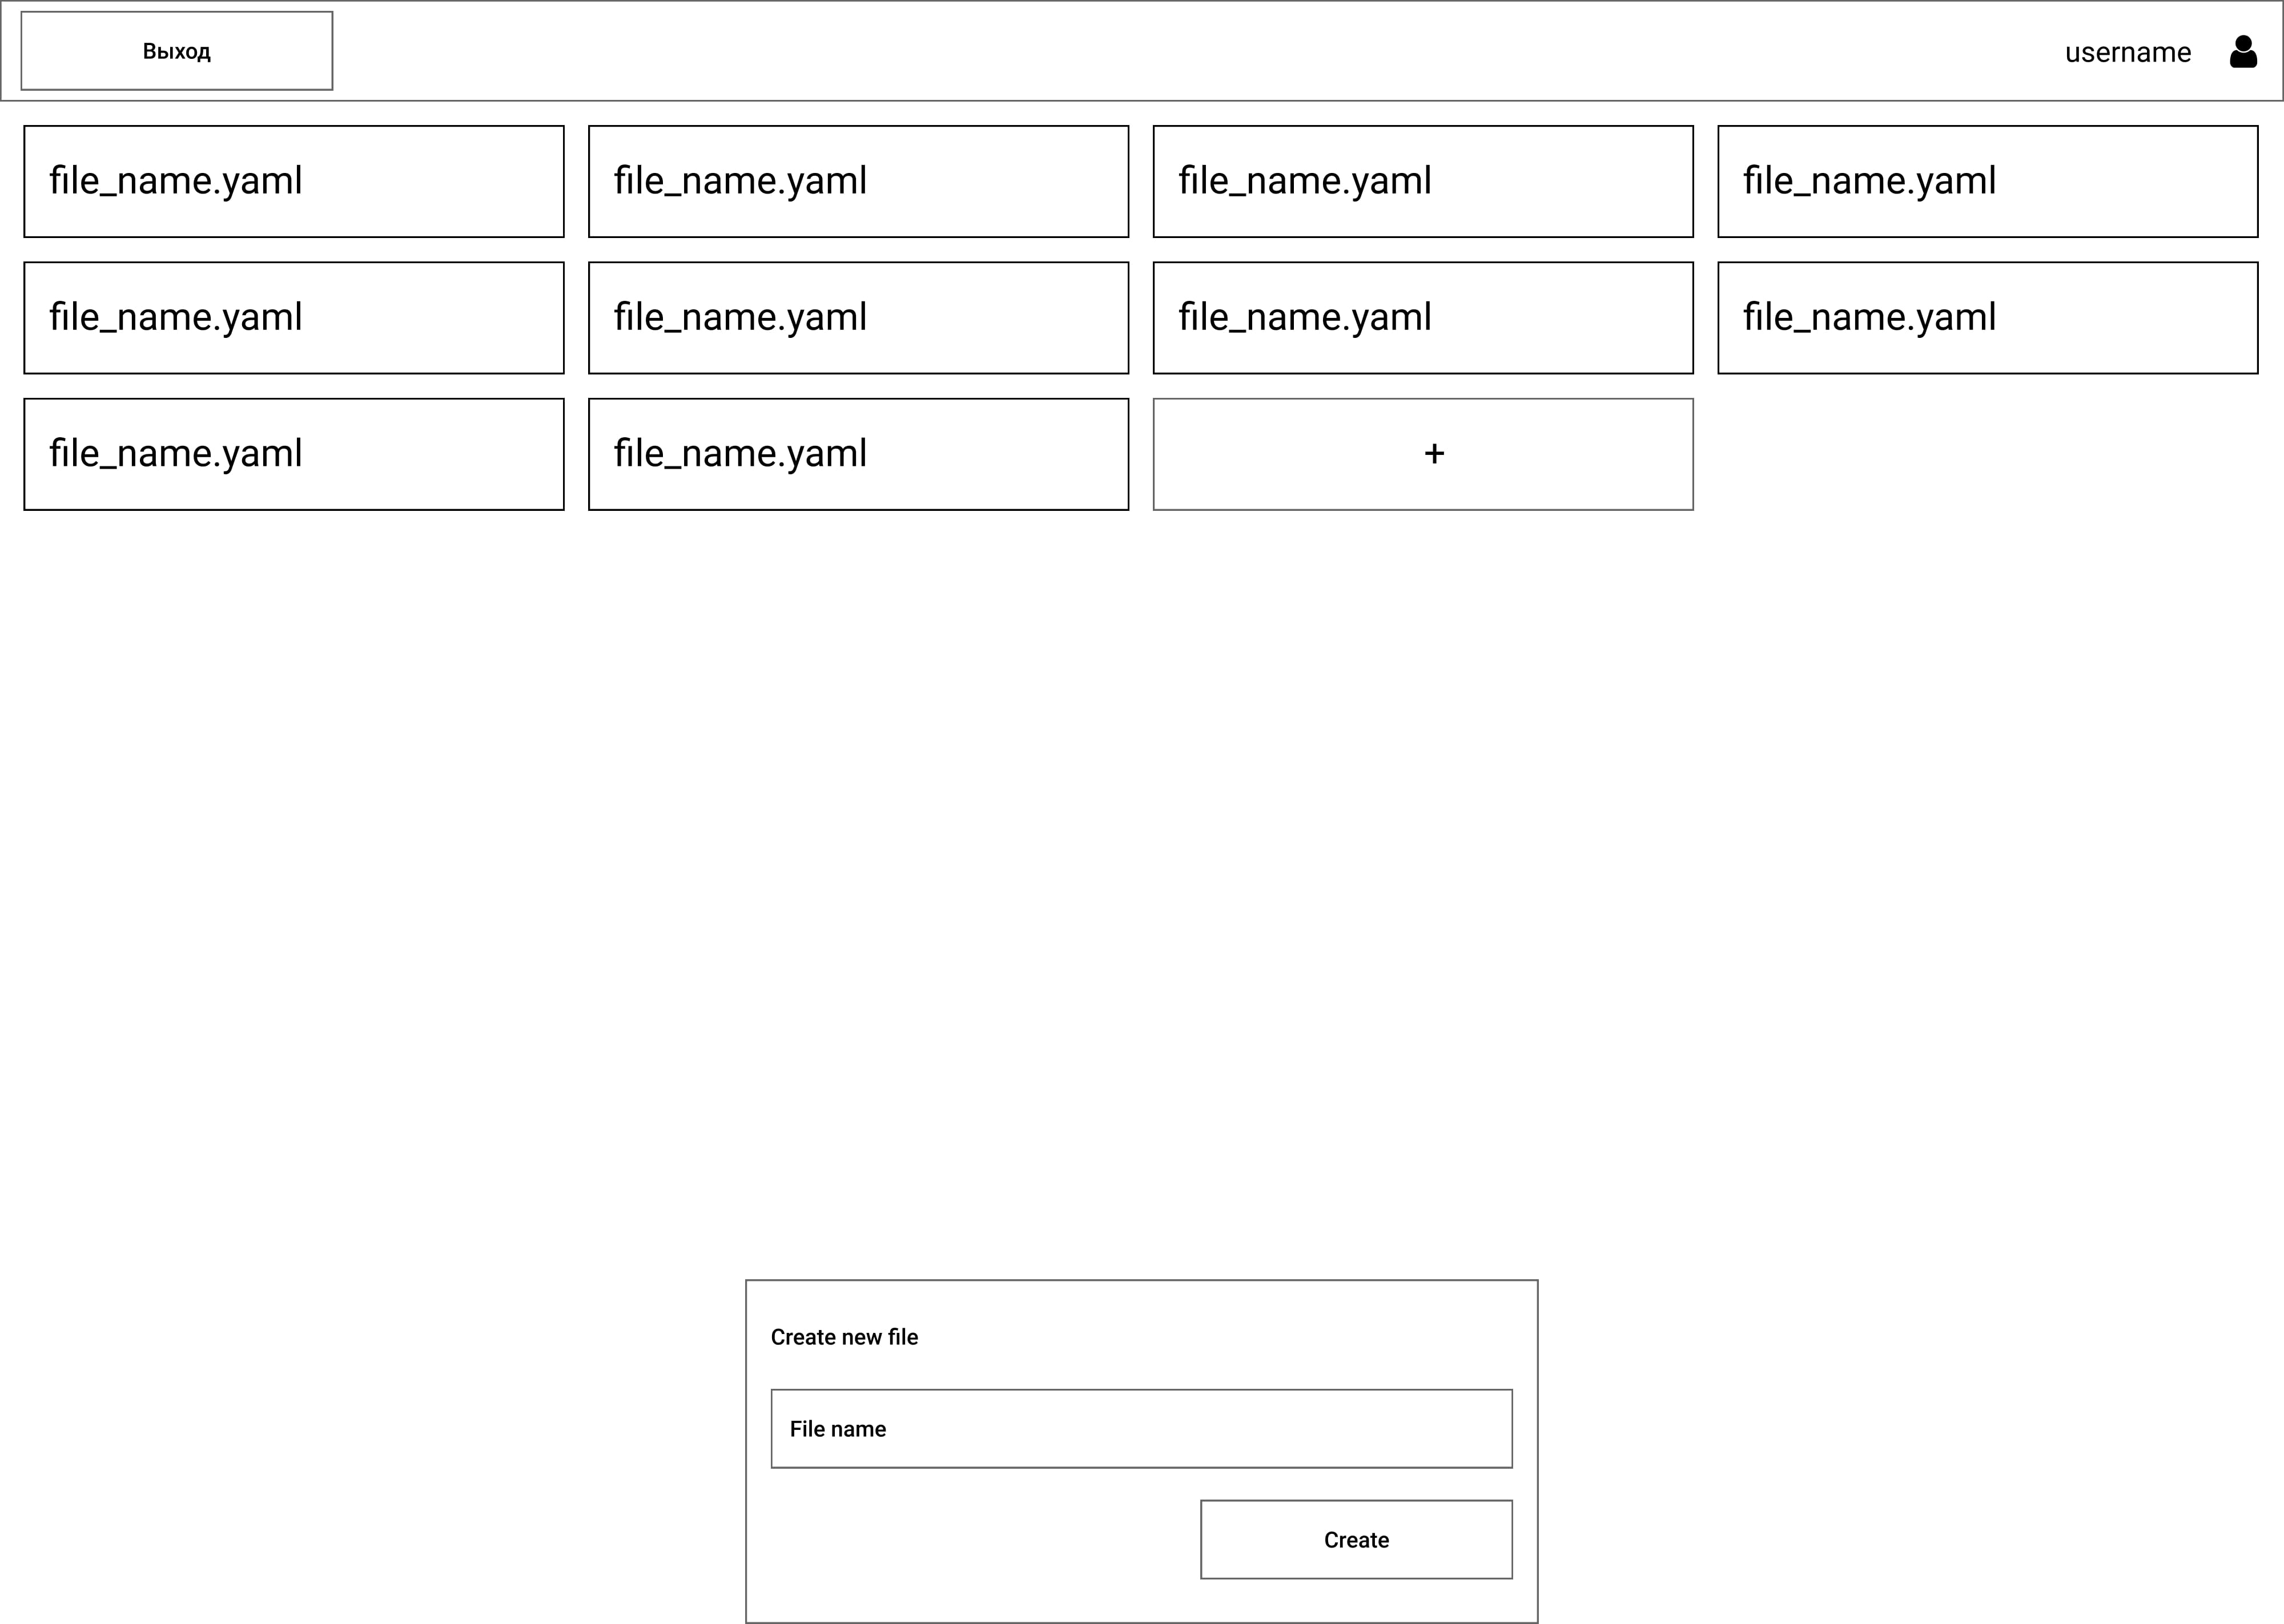
\includegraphics[scale=0.09]{Dashboard.jpg}}
    \caption{Прототип Dashboard-а сайта}
    \label{des:proto_1}
\end{figure}

\begin{figure}[H]
    \center{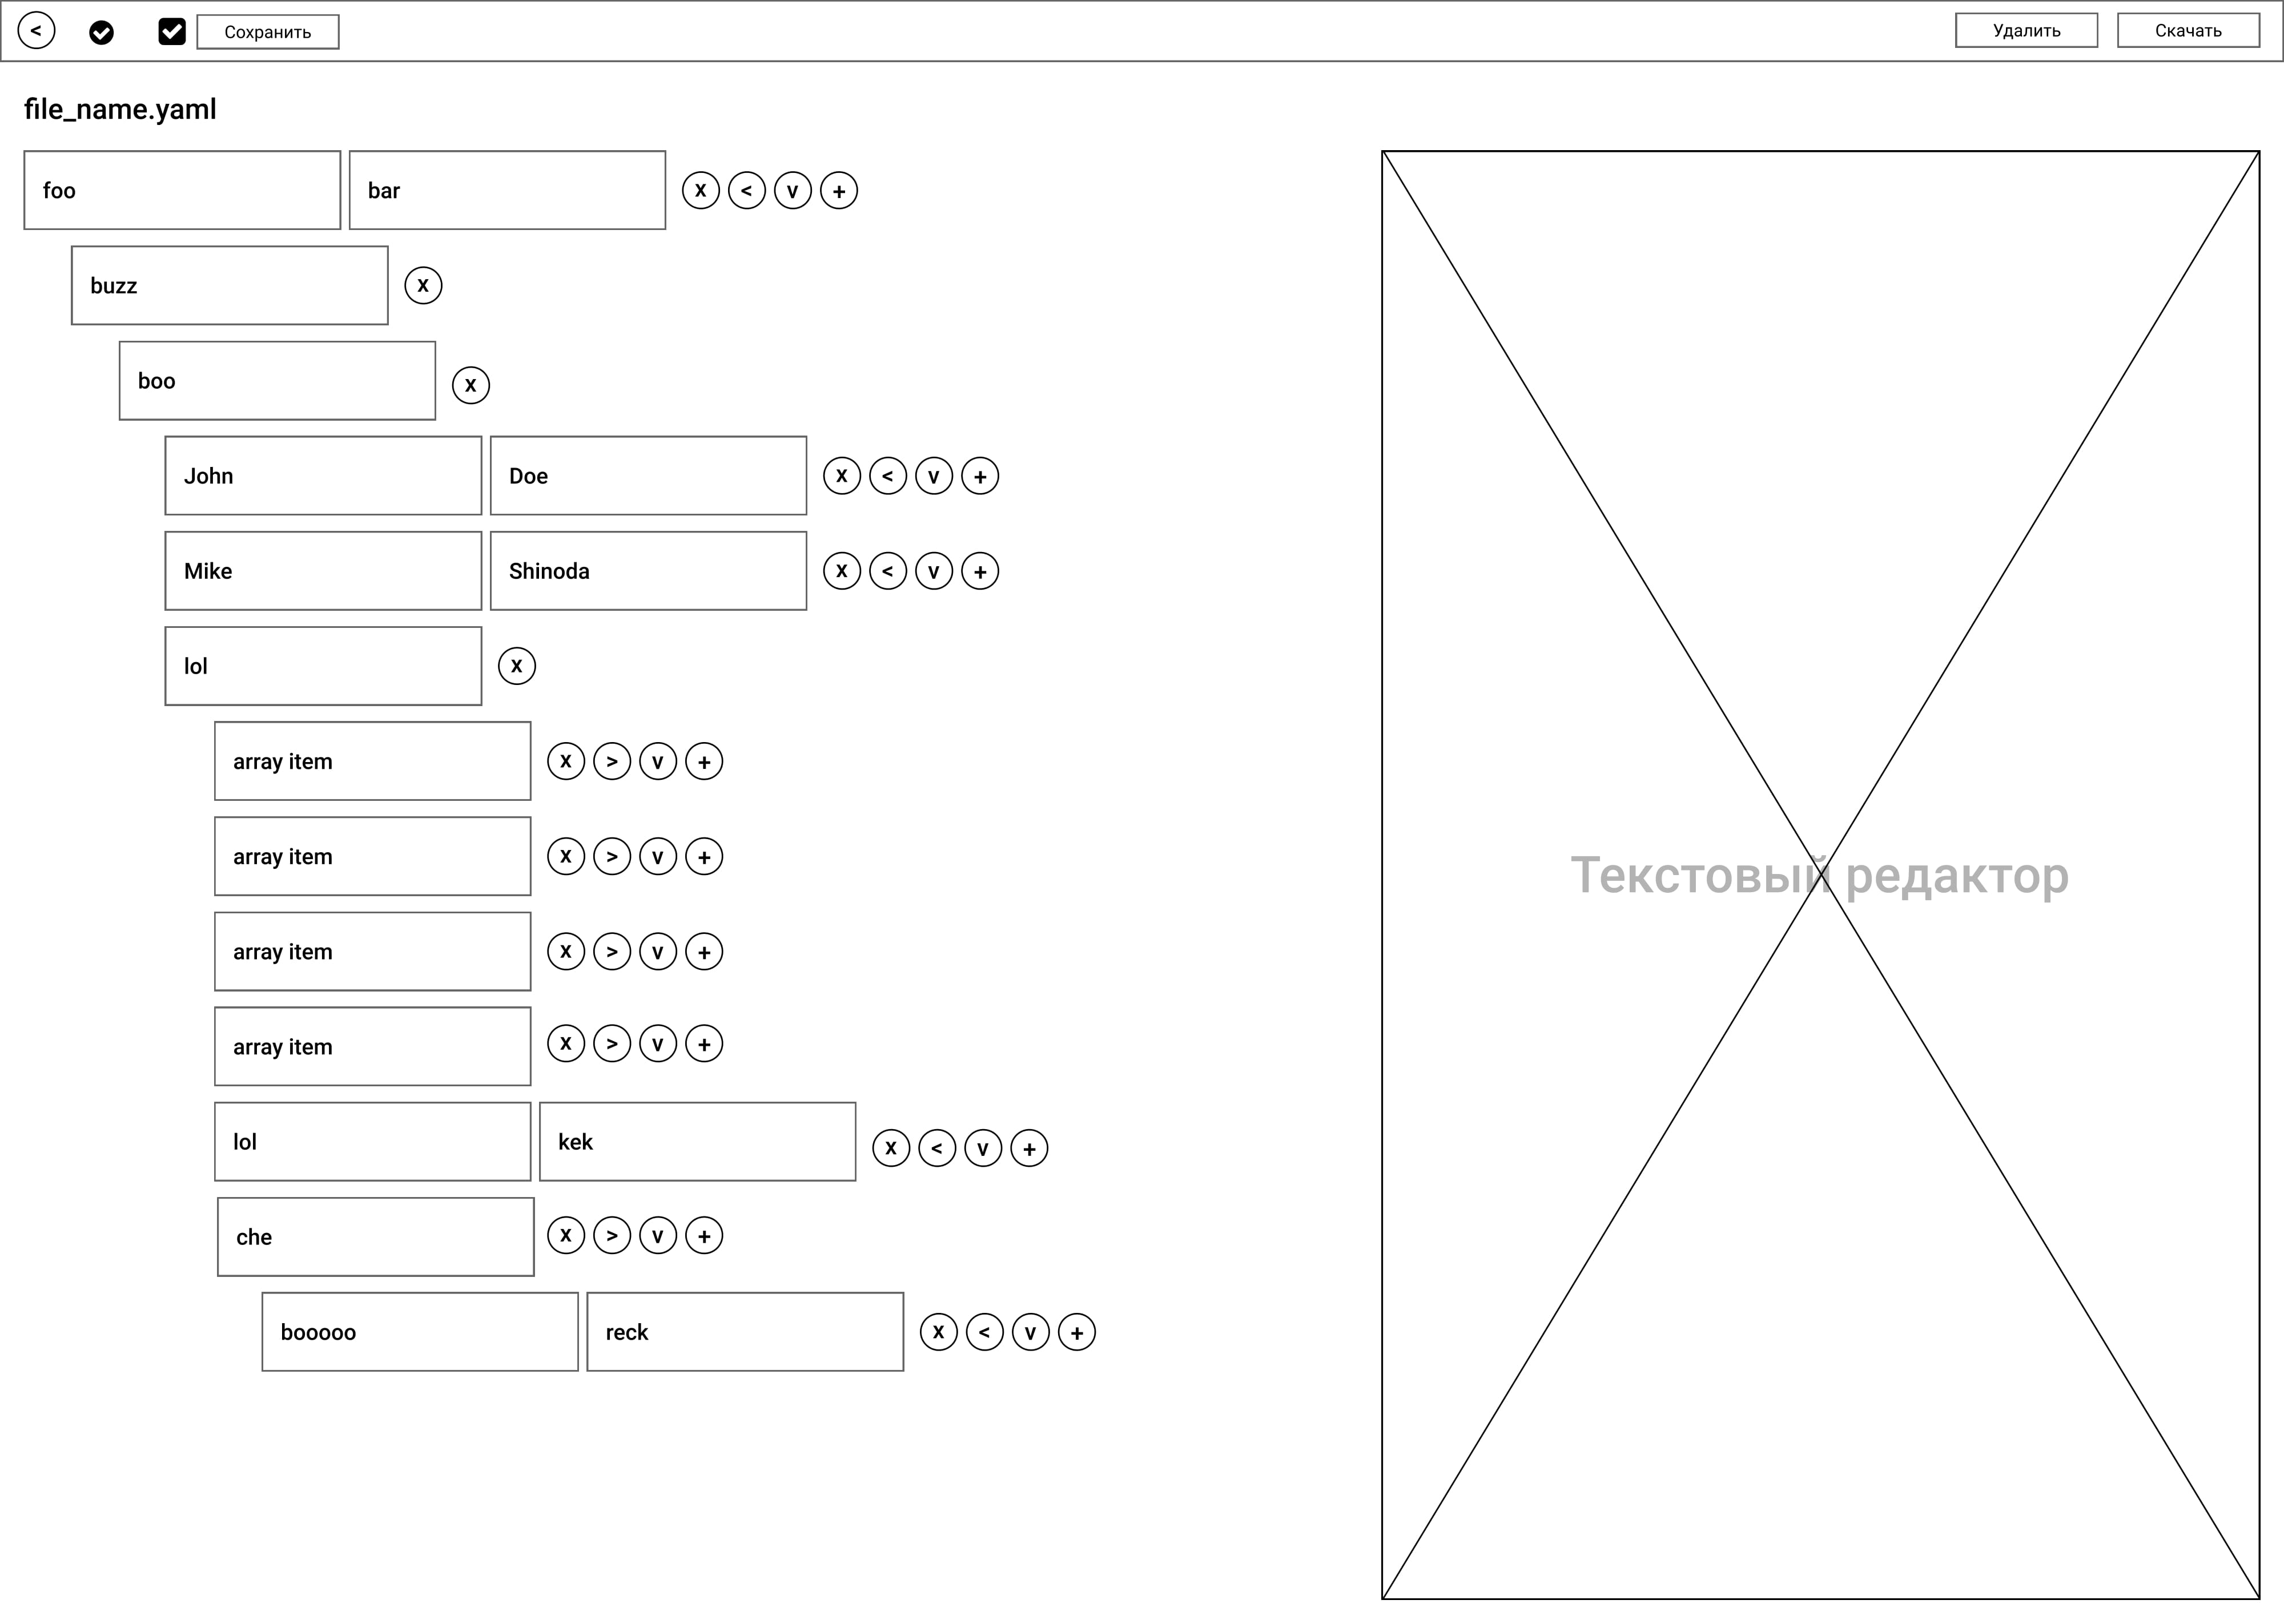
\includegraphics[scale=0.09]{Editor (client).jpg}}
    \caption{Прототип дизайна редактора, если пользователь имеет статус клиента}
    \label{des:proto_2}
\end{figure}

\begin{figure}[H]
    \center{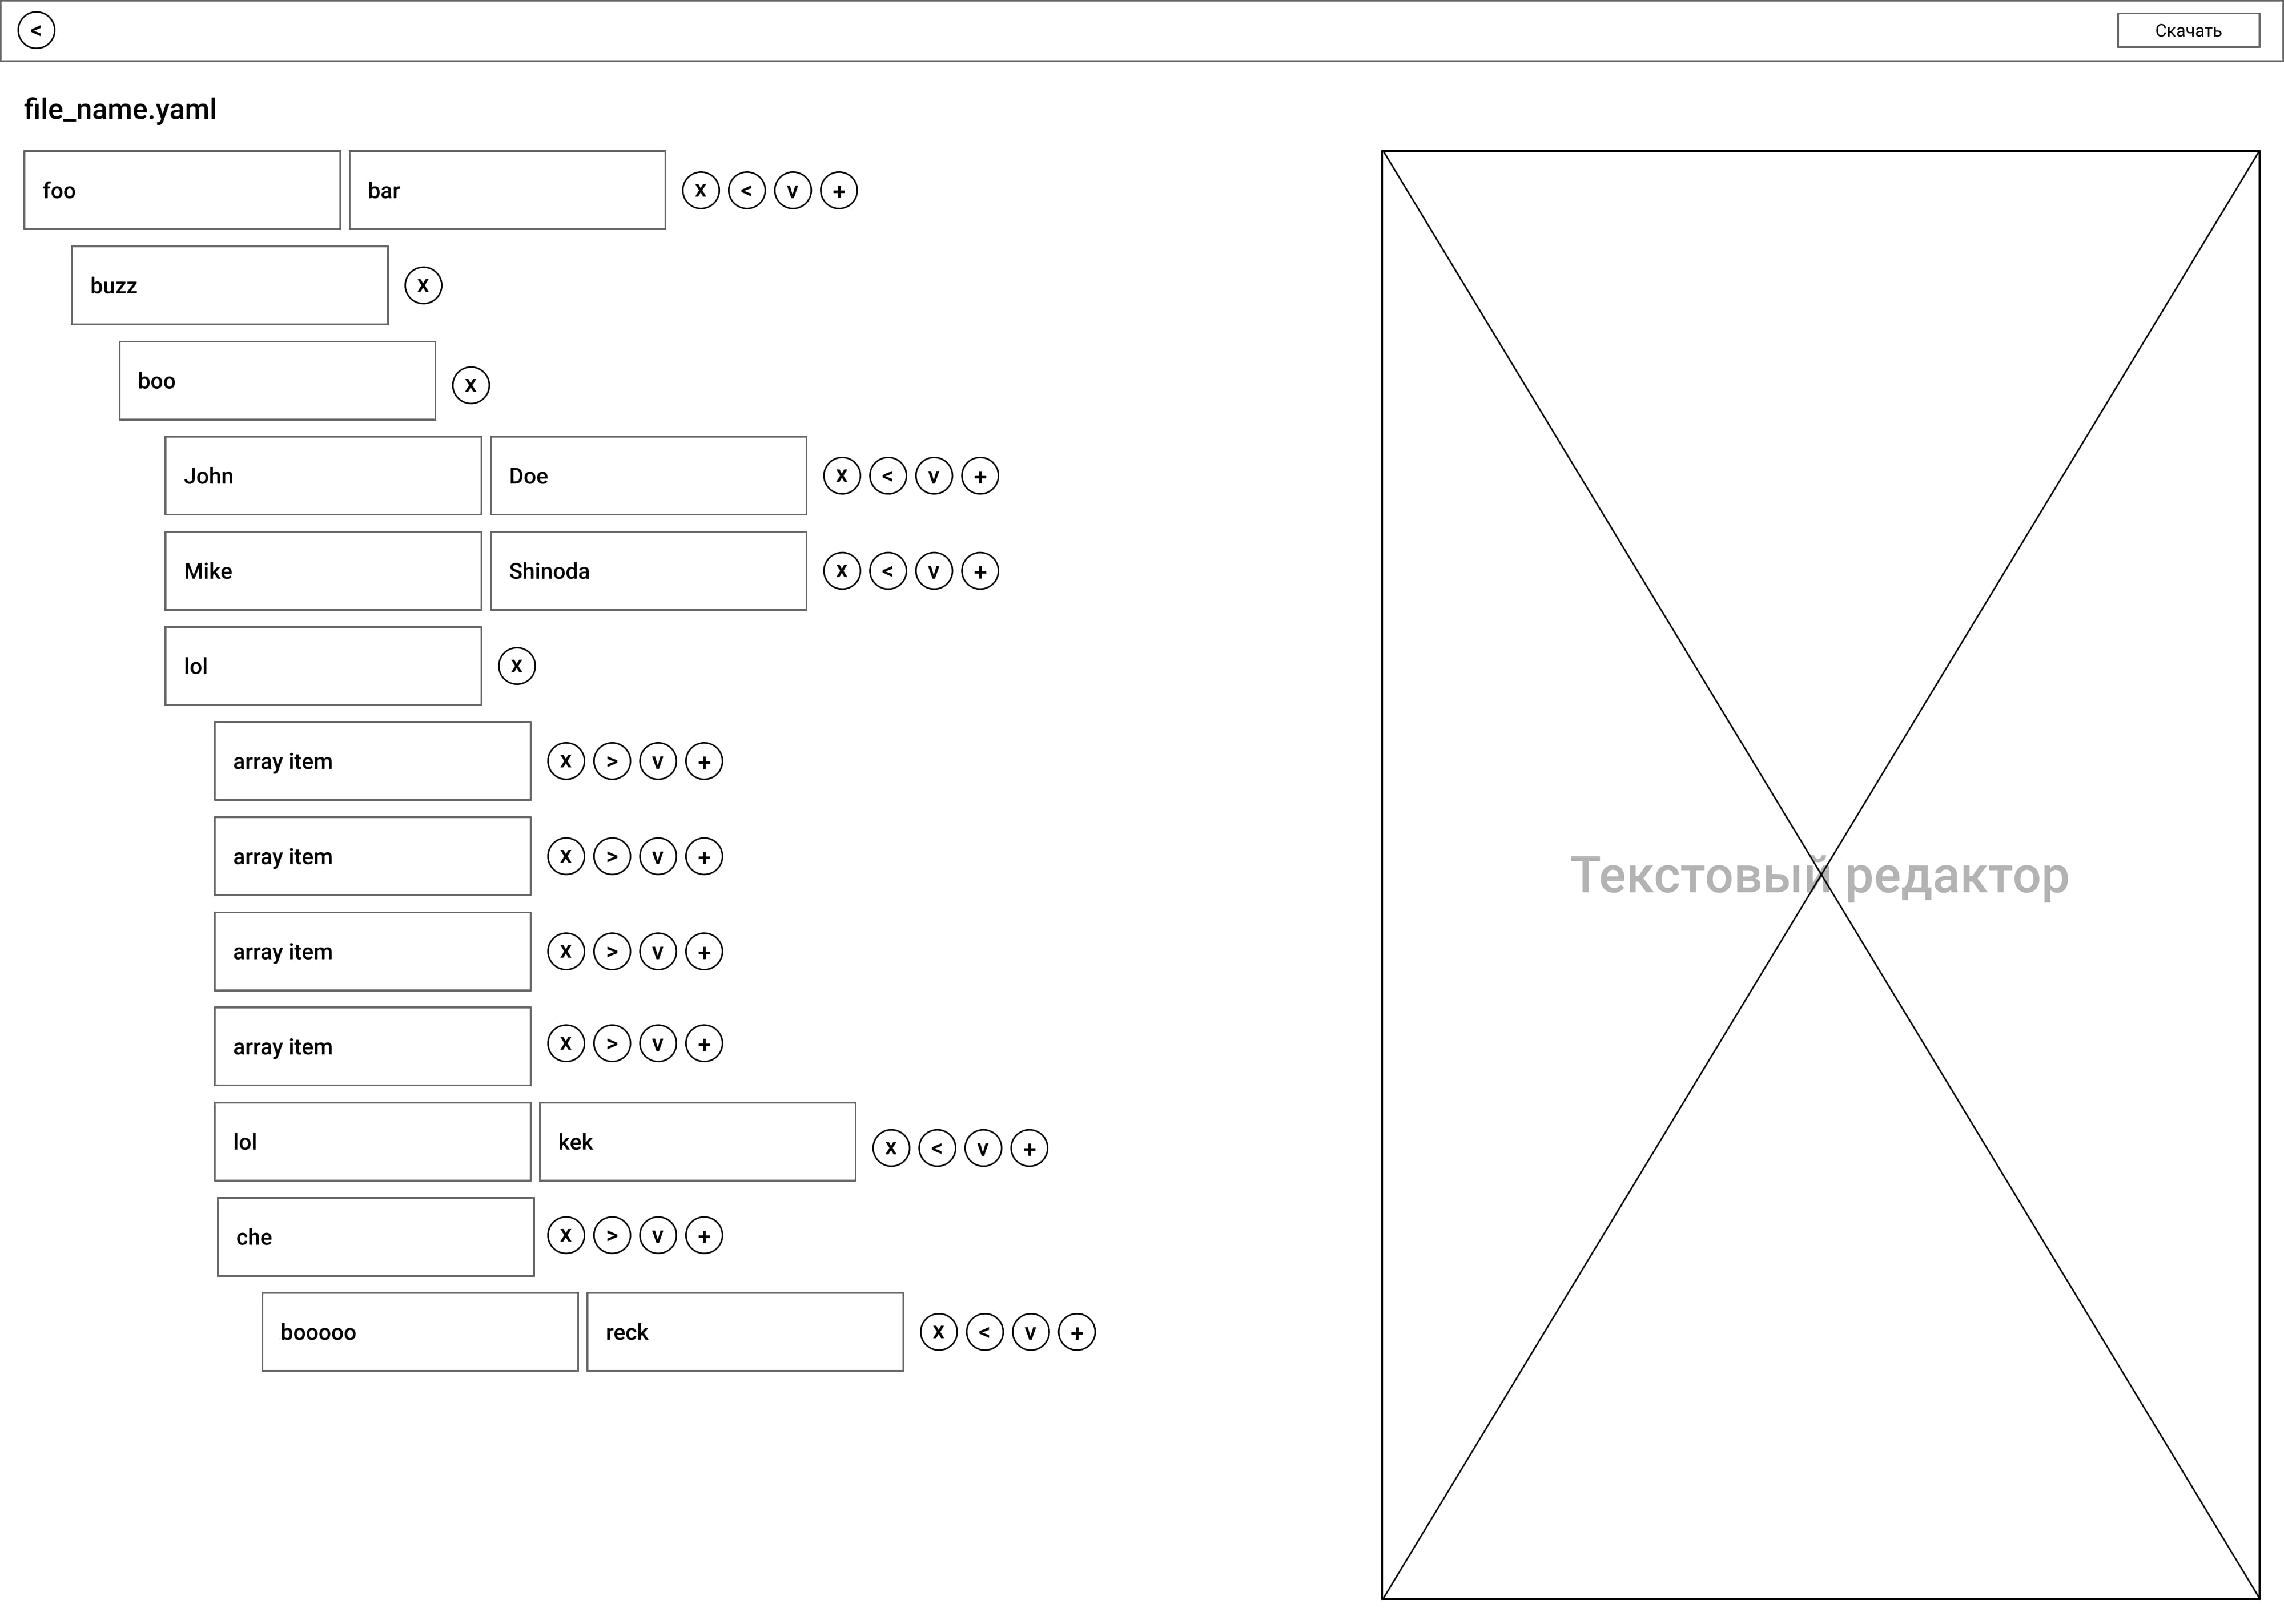
\includegraphics[scale=0.09]{Editor (visitor).jpg}}
    \caption{Прототип дизайна редактора, если пользователь имеет статус посетителя}
    \label{des:proto_3}
\end{figure}

\begin{figure}[H]
    \center{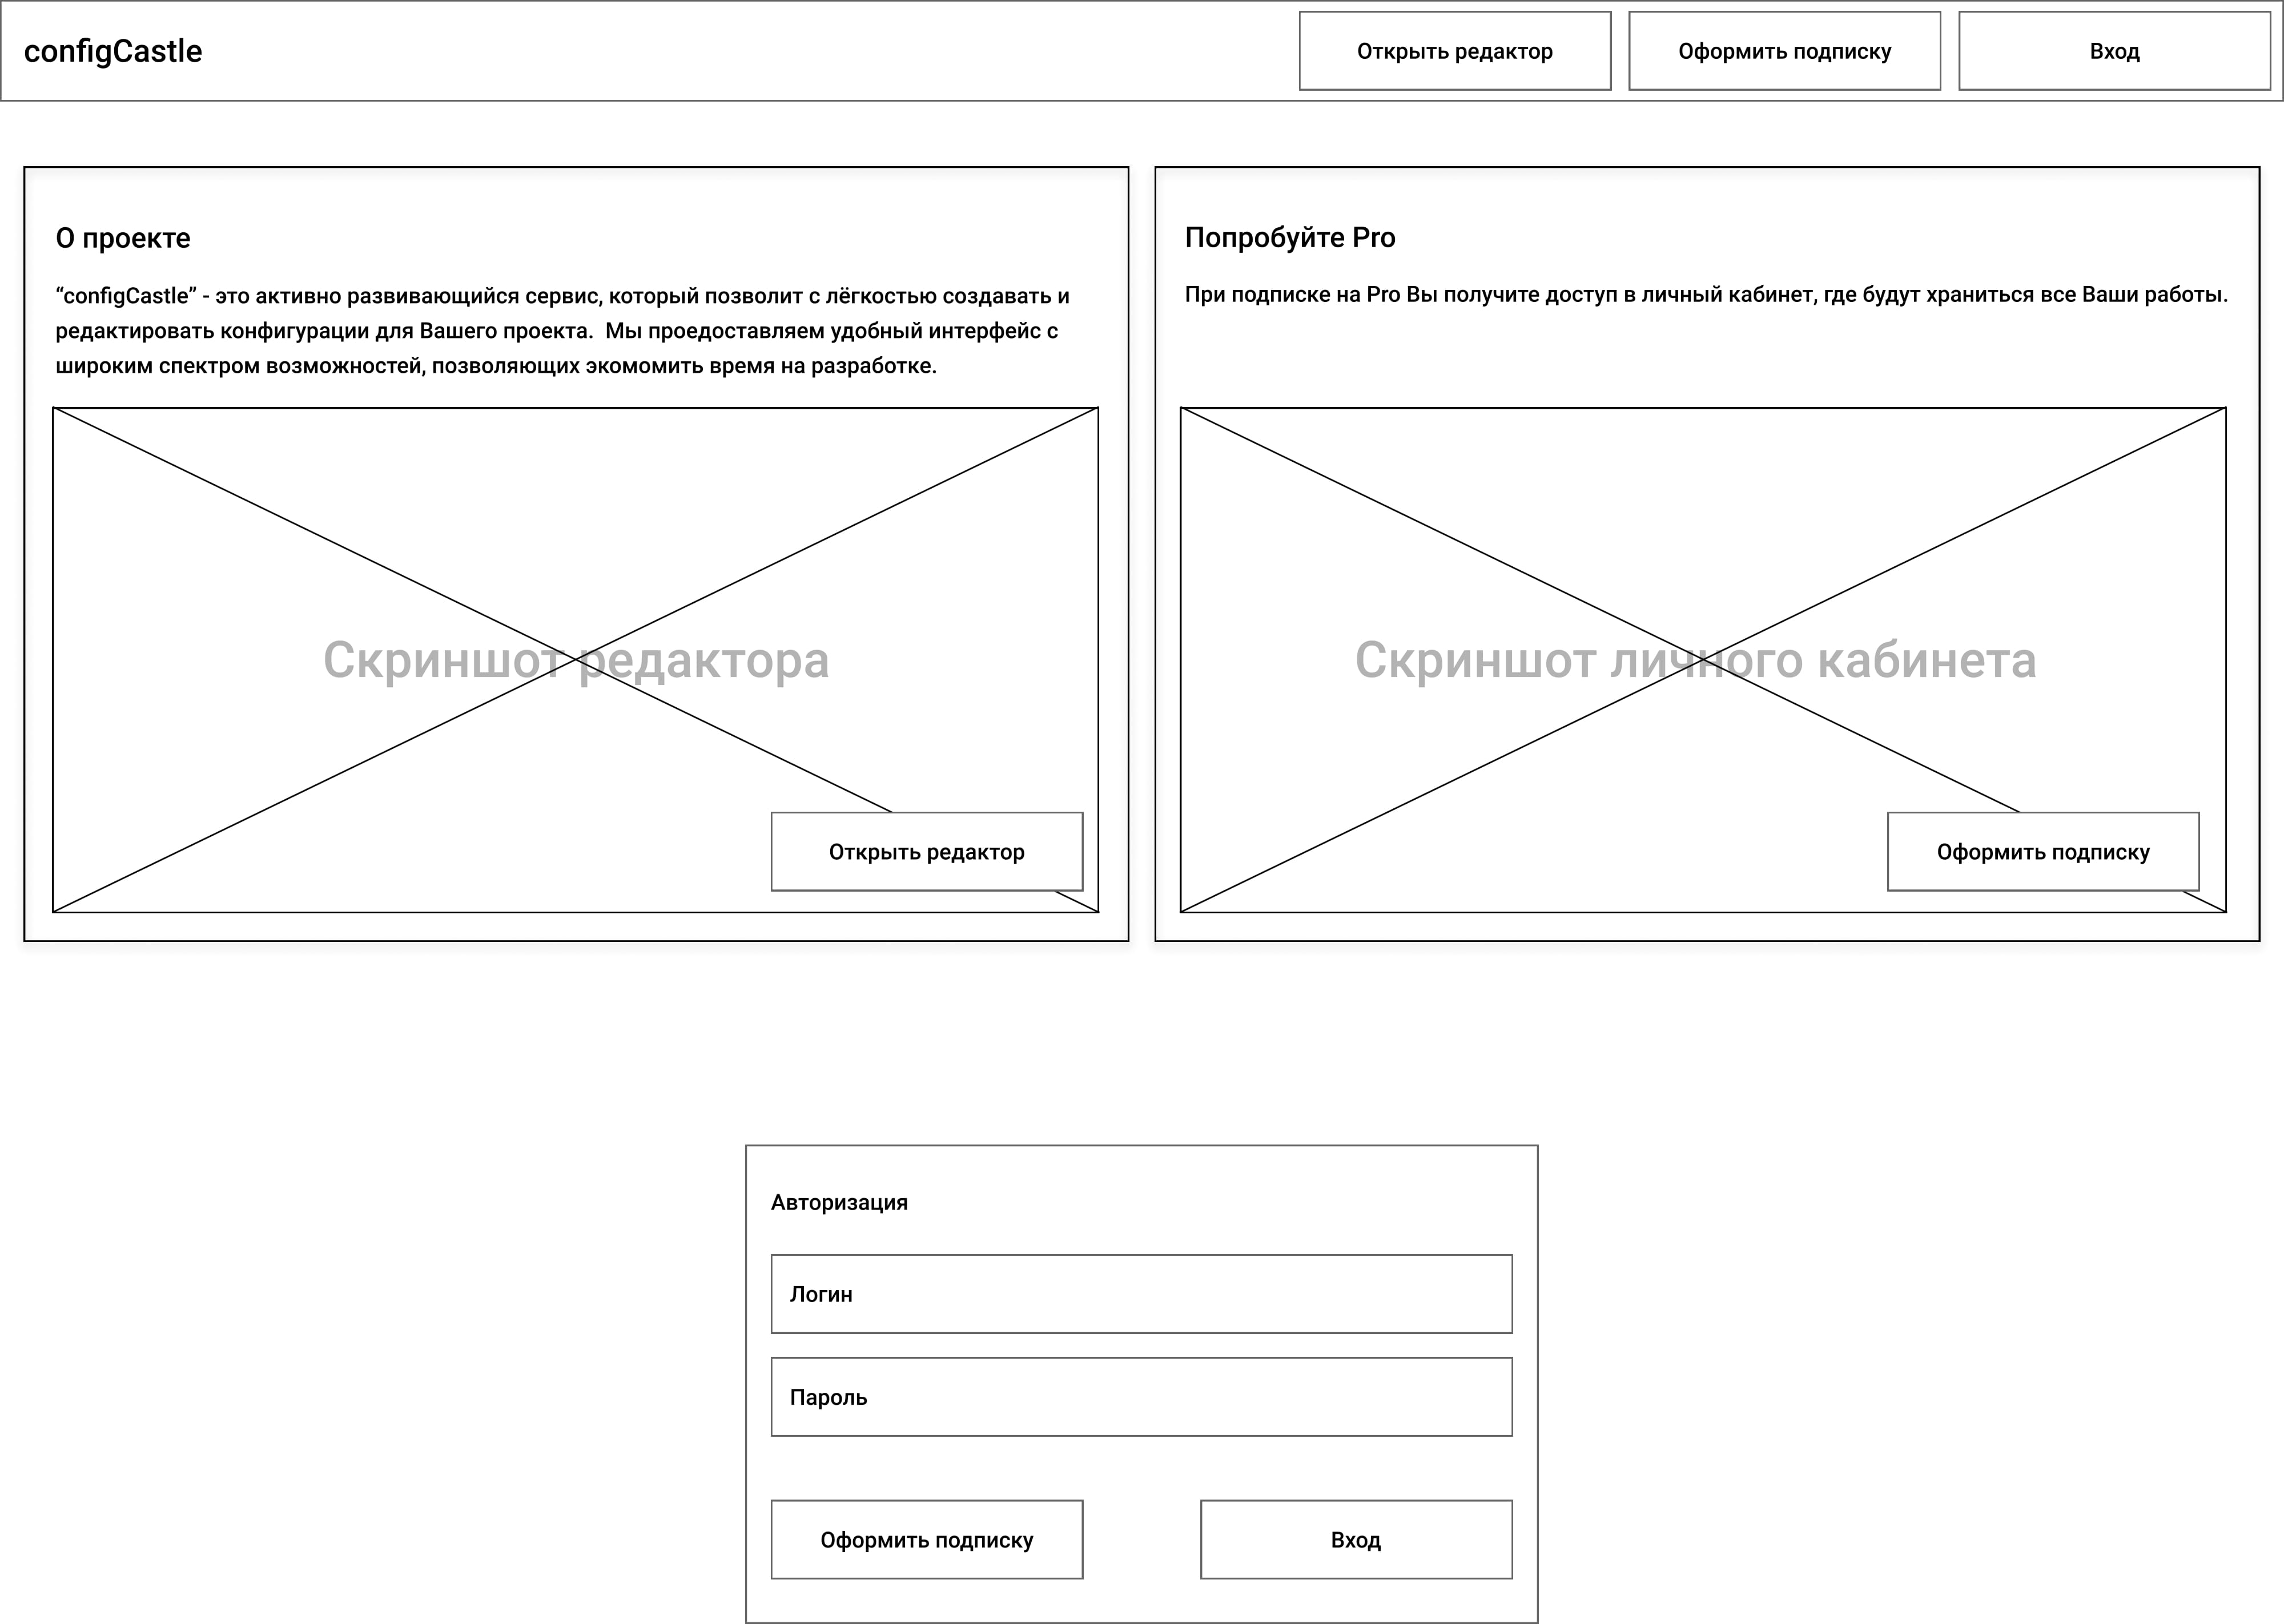
\includegraphics[scale=0.09]{Title (log in).jpg}}
    \caption{Прототип страницы с возможностью входа}
    \label{des:proto_4}
\end{figure}

\begin{figure}[H]
    \center{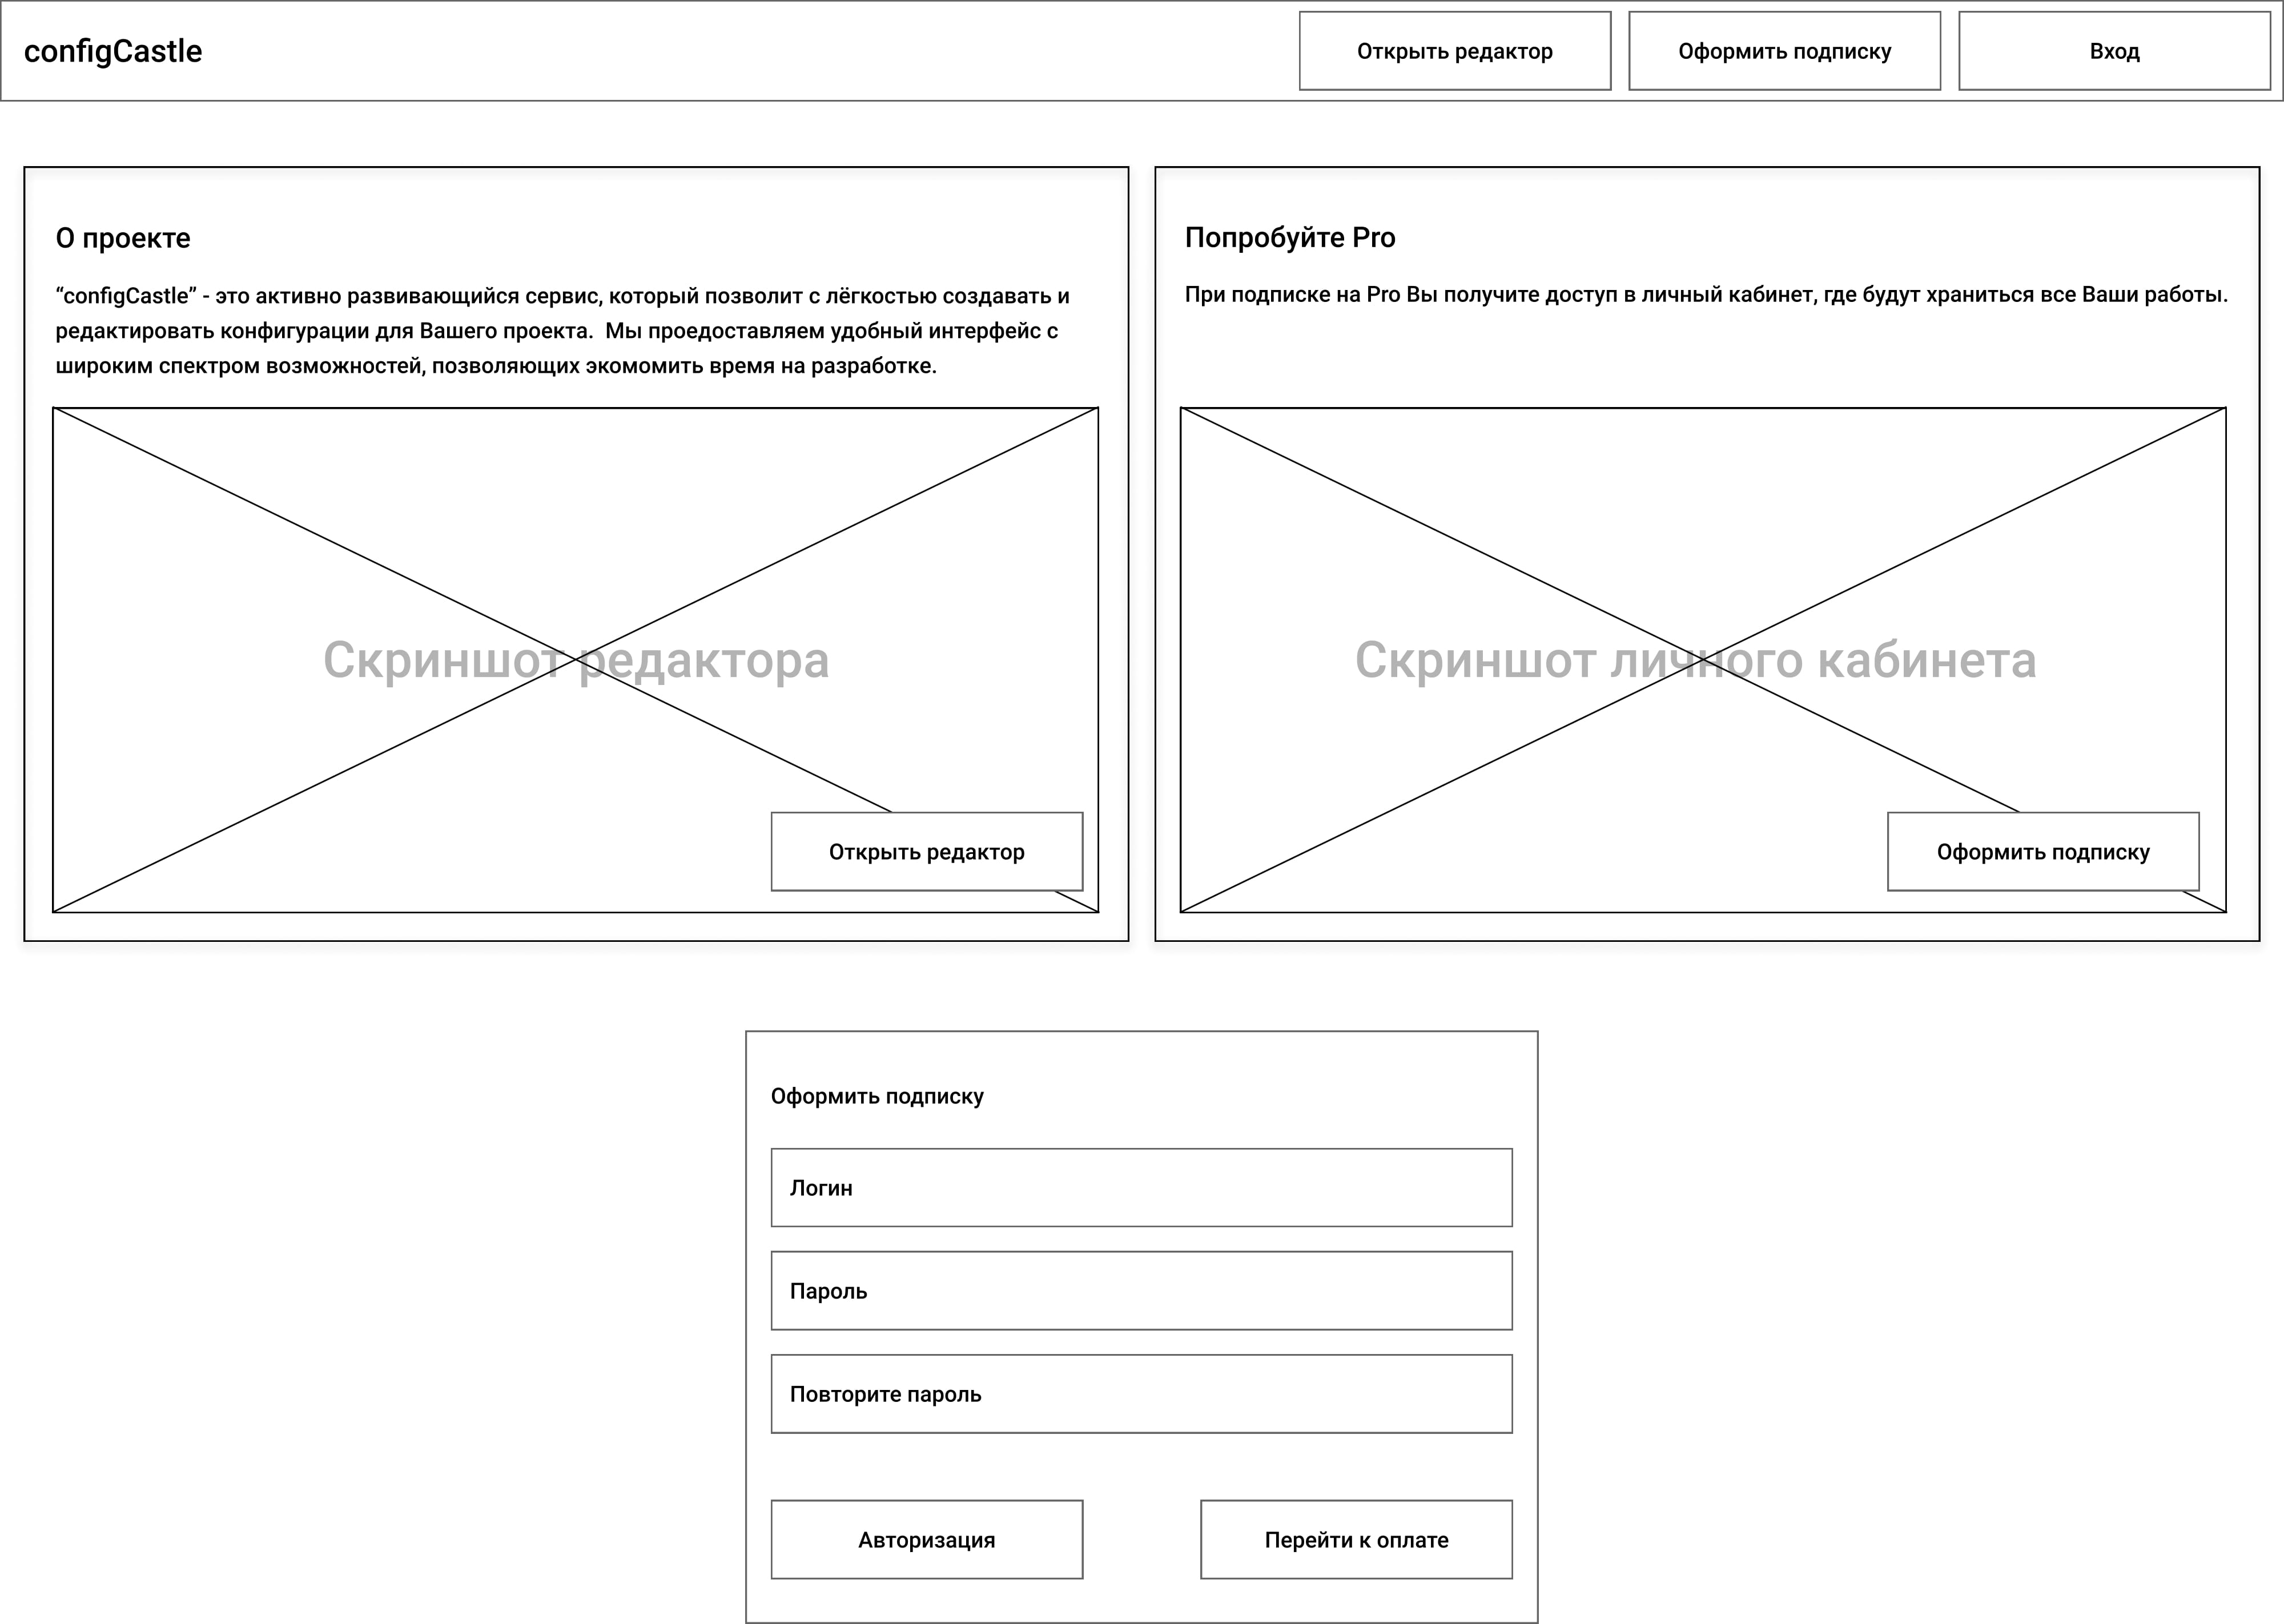
\includegraphics[scale=0.09]{Title (sign in).jpg}}
    \caption{Прототип страницы с возможностю создать аккаунт}
    \label{des:proto_5}
\end{figure}

\begin{figure}[H]
    \center{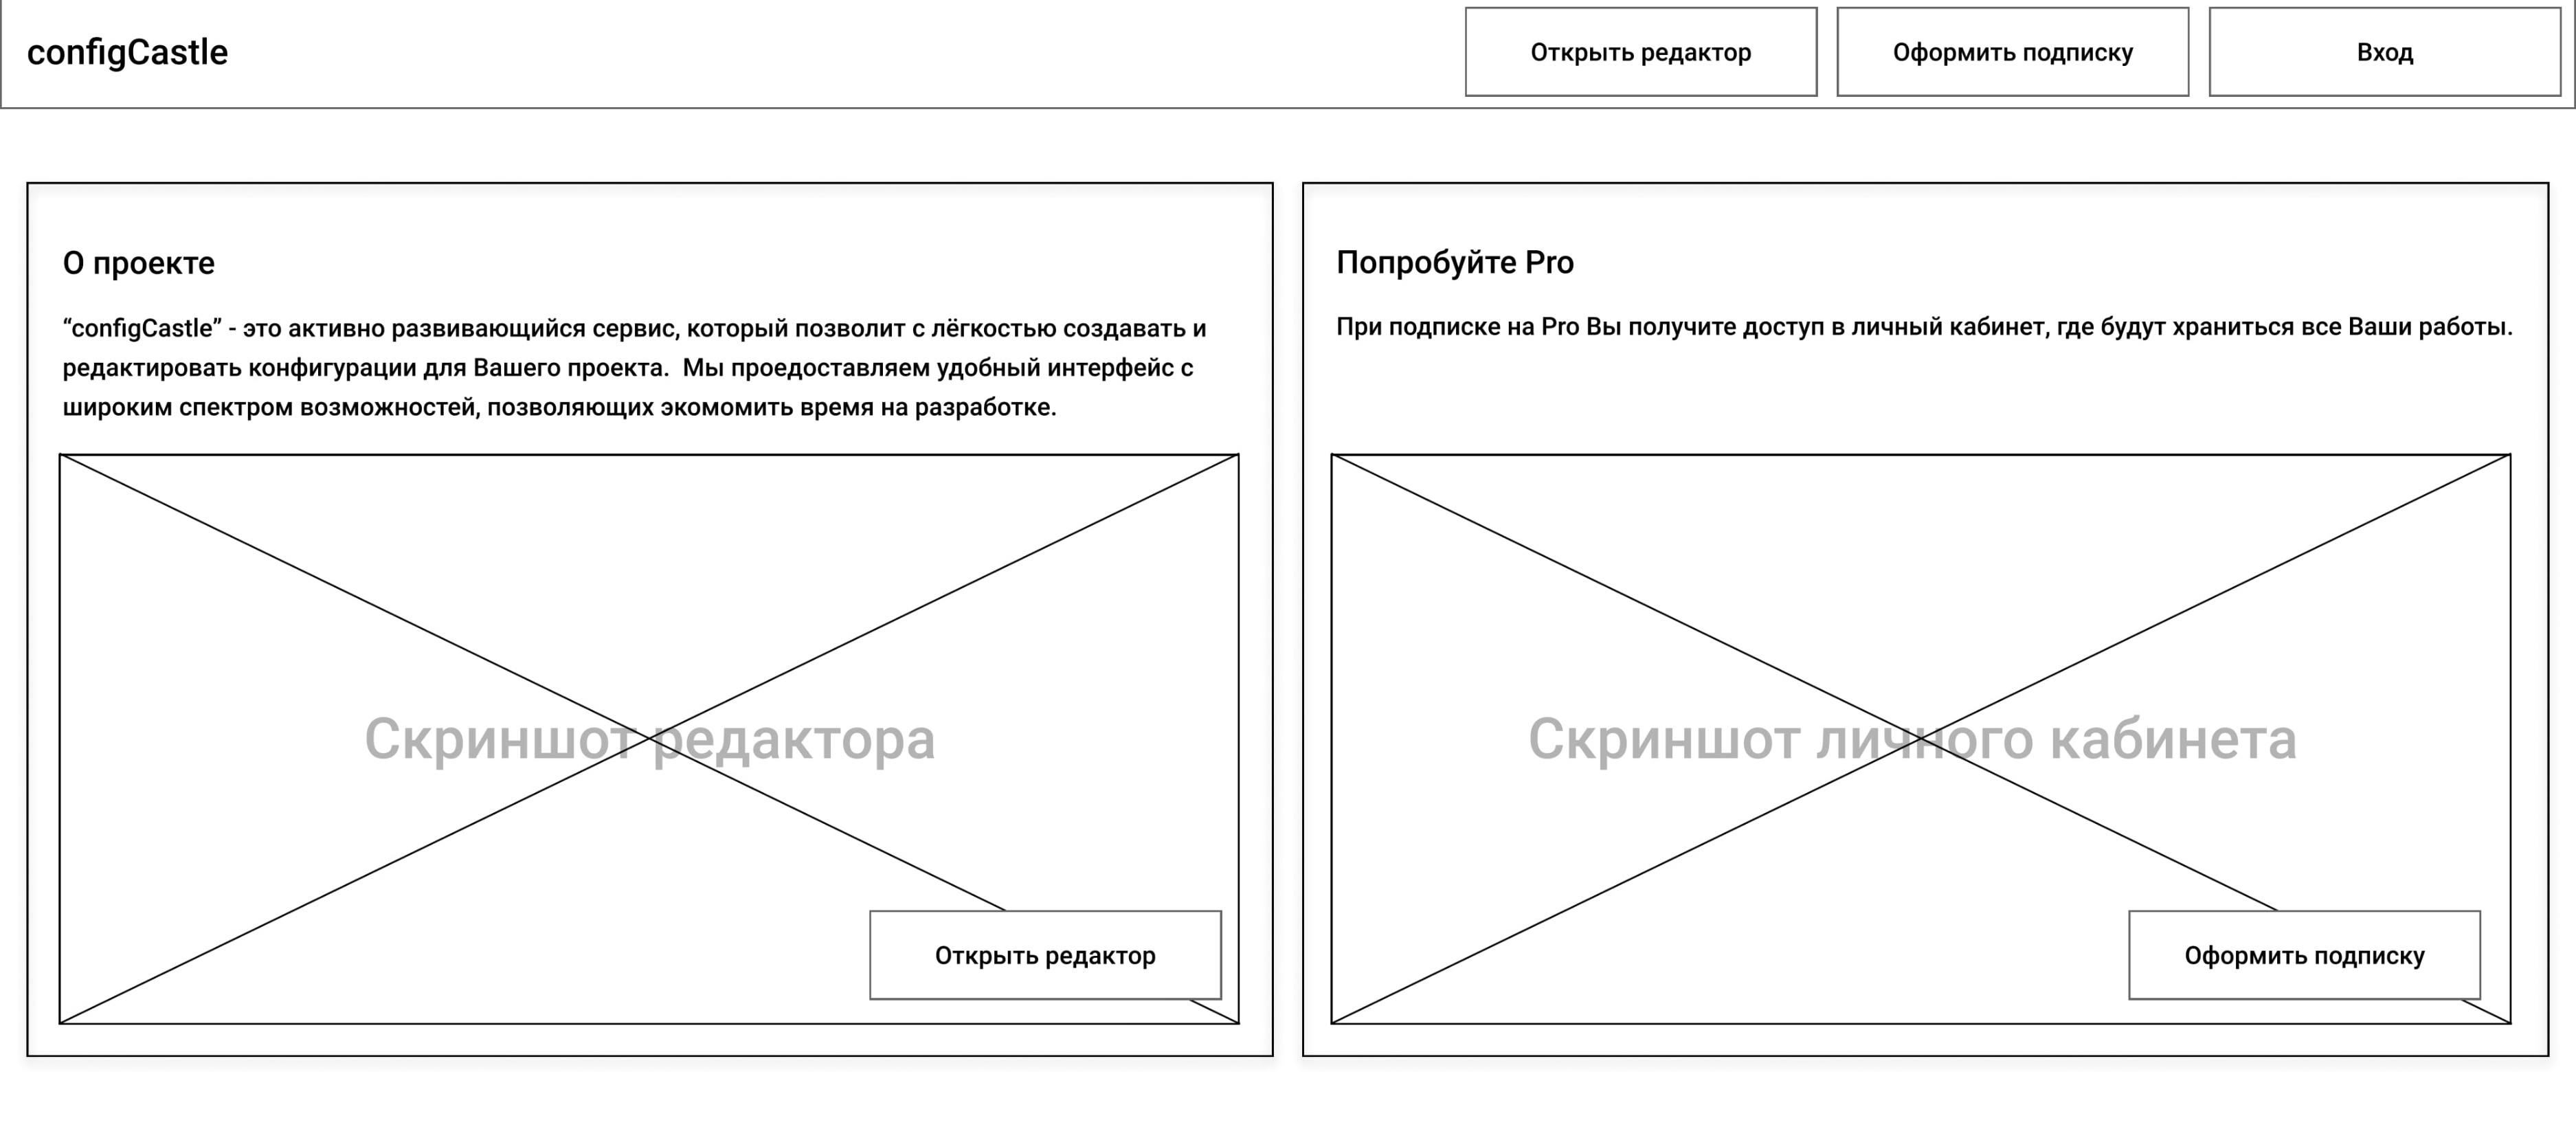
\includegraphics[scale=0.09]{Title.png}}
    \caption{Прототип заглавной страницы}
    \label{des:proto_6}
\end{figure}

\subsection{Архитектура программного продукта}

В ходе проектирования определённое время заняло разработка архитектуры и планирование общего взаимодействия компонентов приложений.

Архитектура программного продукта представляет из себя простой клиент-сервер. Только в этом случае имеется два необщающееся между собой сервера, но имеющие
доступ к одной базе данных, описываемой в разделе \ref{des:bd_section}.

В первую очередь, имеется клиентское приложение. Именно с ним будет взаимодейстовать пользователь: получать с помощью него свои данные, если таковые имеются,
работать с интерфейсом, вносить новые данные и так далее. Сам клиент взаимодействует с двумя серверными частями, которые являются отдельными друг от друга приложениями.

Сервер GraphQL представляет собой серверное приложение, которое необходимо для работы редактора. Оно регистрирует для этого роут и определяет типы для GraphQL, предоставляя
Query и Mutation, которое затем может выполнять и отправлять серверу в виде JSON. Работает непосредственно с базой данной, используя специализированный для этого драйвер.

Сервер авторизации и аутенфикации создан для работы с пользователем. Это приложение не знает о сервере GraphQL, работая независимо, но с той же базой данных, используя
REST API.

База данных хранит информацию о пользователя, созданных файлах и сервисах и нужна для постоянной работы приложения.

Схематично архитектура программного продукта отображена на рисунке \ref{des:arch}.

\begin{figure}[H]
    \center{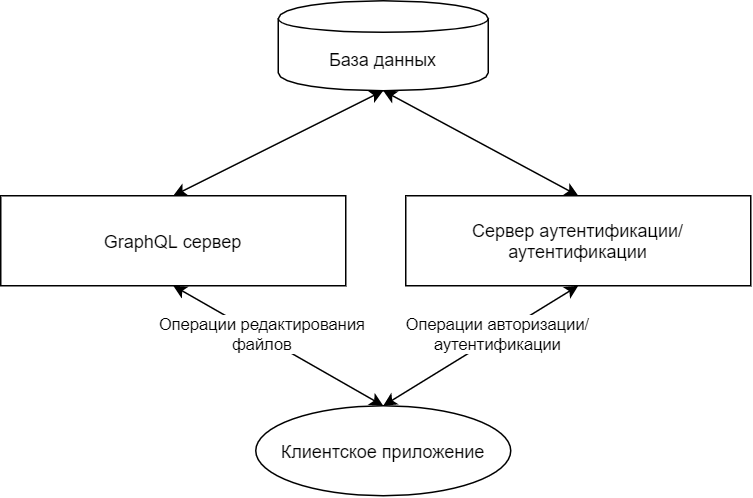
\includegraphics[scale=0.5]{arch.png}}
    \caption{Архитектура проекта}
    \label{des:arch}
\end{figure}

\subsection{Проектирование базы данных}

\label{des:bd_section}

В ходе проекторивания, выбор СУБД остановился на MongoDB. Она позволяет хранить неструктурированные данные в определённых коллекциях в JSON-подобном виде, делая работу с этим форматом удобнее.
Так как потенциально могут возникнуть сервисы с непостоянной структурой, то это делает серверное приложение масшатибируемым, не создаваяя множество миграций. Также для MongoDB имеется
хорошие драйвера, в том числе и асинхронные, что делает этот выбор ещё и производительнее.

Мы имеем определённое количество коллекций, присущих MongoDB ~--- file, service и user, которые хранят соответсвующие данные в виде документов, которые не подчиняются единой
структуре.

На рисунке \ref{des:bd_image} схематично описана структура базы данных.

\begin{figure}[H]
    \center{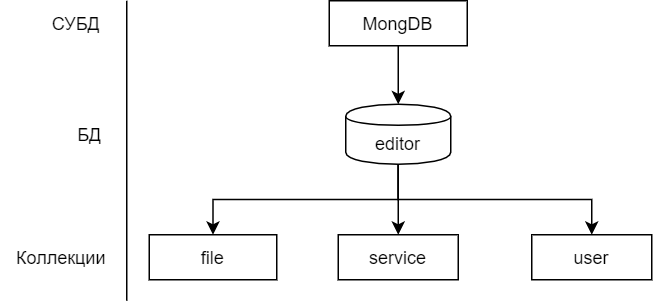
\includegraphics[scale=0.5]{bd.png}}
    \caption{Схематичное описание структуры базы данных}
    \label{des:bd_image}
\end{figure}
